\section{Kivy}
\label{sec:kivy}

\begin{figure}[h]
    \centering
    
\includegraphics[scale=0.5]{images/chapter3/kivy_logo.png}
    \caption{Kivy}
\end{figure}

Το Kivy\footnote{\href{https://kivy.org/}{https://kivy.org/}} είναι μια βιβλιοθήκη ανοιχτού κώδικα της Python για την γρήγορη ανάπτυξη εφαρμογών που χρησιμοποιούν γραφικά για υλοποίηση καινοτόμων διεπαφών χρηστών. Επιλέξαμε την εν λόγω βιβλιοθήκη για την υλοποίηση της διεπαφής του καθρέφτη επειδή είναι:
\begin{itemize}
    \item \textbf{Cross Platform:} Το Kivy τρέχει σε διαφορετικά λειτουργικά συστήματα και πλατφόρμες όπως Windows, Linux, Android, OS X, Raspberry Pi με τον ίδιο κώδικα.
    \item \textbf{GPU Accelerated:} Η μηχανή γραφικών έχει υλοποιηθεί πάνω στην OpenGL ES 2 χρησιμοποιώντας μια σύγχρονη και γρήγορη γραμμή γραφικών.
    \item \textbf{Εύκολη στη Χρήση:} Περιλαμβάνει μια ευρεία γκάμα έτοιμων widgets ενώ χρησιμοποιεί μια απλή ενδιάμεση γλώσσα (kv) για τον εύκολο σχεδιασμό widget από τον χρήστη.
\end{itemize}

\subsection{Αρχιτεκτονική του Kivy}
Το Kivy αποτελείται από πολλά δομικά κομμάτια όπως φαίνεται στο Σχήμα \ref{fig:kivy_arch}. Κάποια βασικά από αυτά τα δομικά κομμάτια περιγράφονται στη συνέχεια \cite{kivy}.

\begin{figure}[ht]
    \centering
    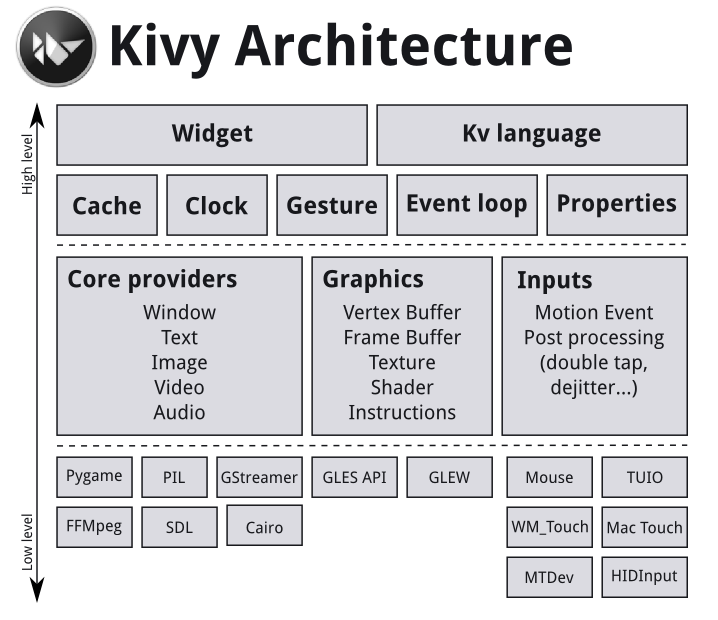
\includegraphics[scale=0.5]{images/chapter3/kivy_architecture.png}
    \caption{Αρχιτεκτονική της βιβλιοθήκης Kivy}
    \label{fig:kivy_arch}
\end{figure}

\subsubsection{Core και Input Providers}
Ένας Core Provider είναι ένα κομμάτι κώδικα που λειτουργεί ως διαμεσολαβητής ανάμεσα στο ΛΣ και το Kivy. Η βασική ιδέα είναι να χωριστούν εργασίες όπως το άνοιγμα ενός παραθύρου, η εμφάνιση μια εικόνας ή κειμένου, η αναπαραγωγή ήχου κτλ. έτσι ώστε το API να είναι εύχρηστο και επεκτάσιμο. Το βασικότερο πλεονέκτημα όμως είναι ότι με αυτόν τον τρόπο επιτρέπεται να χρησιμοποιηθούν συγκεκριμένοι providers ανάλογα με τα σενάρια χρήσης της εφαρμογής. Για παράδειγμα, τα OS X, Linux και Windows χρησιμοποιούν διαφορετικούς providers για τις παραπάνω εργασίες. Με τη χρήση εξειδικευμένων providers για κάθε πλατφόρμα είναι εφικτή η πλήρης αξιοποίηση του ΛΣ με αποδοτικό τρόπο, ενώ είναι εφικτή η μεταφορά της εφαρμογής σε άλλες πλατφόρμες αρκετά εύκολα.

Με αντίστοιχο τρόπο δουλεύουν και οι providers εισόδων. Αν κάποιος θέλει να υποστηρίξει μια νέα συσκευή εισόδου χρειάζεται απλά να γράψει μία κλάση η οποία διαβάζει τα δεδομένα της συγκεκριμένης συσκευής και τα μεταφράζει και γεγονότα του Kivy (Kivy Events).

\subsubsection{Γραφικά}
Το γραφικό API του Kivy είναι μια αφαιρετικότητα της OpenGL. Στο χαμηλότερο επίπεδο το Kivy δίνει hardware accelerated εντολές σχεδιασμού χρησιμοποιώντας OpenGL. Αλλά επειδή το να γράφει κανείς σε OpenGL είναι επίπονο, ειδικά για τους νέους χρήστες, είναι εφικτό να σχεδιαστού γραφικά χρησιμοποιώντας μεταφορικές εντολές (Canvas, Rectangle κτλ.) που δεν υπάρχουν στην OpenGL.  

\subsubsection{Πυρήνας}
Ο κώδικας του πακέτου του πυρήνα παρέχει συχνά χρησιμοποιούμενα χαρακτηριστικά όπως:
\begin{itemize}
    \item Το \textbf{ρολόι} που χρησιμοποιείται για να προγραμματιστούν χρονικά γεγονότα.
    \item Την \textbf{cache} σε περίπτωση που κάποιος θέλει να αποθηκεύσει κάτι που χρησιμοποιείται συχνά.
    \item Την \textbf{αναγνώριση χειρονομίας} για αποθήκευση και ανίχνευση διαφόρων σχημάτων, όπως κύκλοι, ενώ μπορεί να εκπαιδευτεί για σχήματα που καθορίζει ο χρήστης.
    \item Την \textbf{γλώσσα Kivy} η οποία χρησιμοποιείται για να περιγραφούν με ευκολία και αποδοτικότητα οι διεπαφές χρηστών
    \item Τις \textbf{ιδιότητες} οι οποίες είναι κλάσεις που συνδέουν τον κώδικα ενός widget με την περιγραφή της διεπαφής του χρήστη.
\end{itemize}

\subsubsection{UIX}
Το συγκεκριμένο πακέτο περιέχει τα πιο συχνά χρησιμοποιούμενα widgets και layouts για την γρήγορη ανάπτυξη μια διεπαφής χρήστη.
\begin{itemize}
    \item Τα \textbf{widgets} είναι στοιχεία διεπαφής τα οποία εισάγονται στο πρόγραμμα και παρέχουν κάποια λειτουργία όπως πχ. κουμπιά, λίστες, επιγραφές κ.α.
    \item Τα \textbf{layouts} χρησιμοποιούνται για την διάταξη των widgets.
\end{itemize}